\documentclass[11pt, a4paper]{article}
\usepackage[margin=2.5cm]{geometry}
\usepackage{graphicx}
\usepackage{amsmath, amssymb}
\usepackage{booktabs}
\usepackage{caption}
\usepackage{subcaption}
\usepackage{hyperref}
\usepackage{float}

\graphicspath{{../Figures/}}

\title{\textbf{Task 1: Simulation and Sensitivity Analysis of Chaotic Systems}}
\author{Ibrahim Hanafy}
\date{July 2026}

\begin{document}
\maketitle

%% ===== PART A =====
\section{Part A --- Discrete Chaotic Systems}

\subsection{Logistic Map}

The logistic map $x_{n+1} = r \cdot x_n (1 - x_n)$ was iterated for 1000 steps with $x_0 = 0.5$. At $r = 3.9$ (chaotic regime), the time series exhibits aperiodic oscillations bounded within $[0, 1]$, characteristic of deterministic chaos.

\begin{figure}[H]
    \centering
    
\includegraphics[width=0.85\textwidth]{logistic_timeseries.png}
    \caption{Logistic map time series at $r = 3.9$.}
    \label{fig:logistic_ts}
\end{figure}

The bifurcation diagram (Fig.~\ref{fig:logistic_bif}) sweeps $r \in [2.5, 4.0]$ with 2000 values, discarding the first 500 transient iterations. A clear period-doubling cascade is visible: the system transitions from a stable fixed point ($r < 3$) through successive period-doublings ($r \approx 3.0, 3.45, 3.54$) into full chaos ($r \gtrsim 3.57$). Periodic windows (e.g., the period-3 window near $r \approx 3.83$) appear embedded within the chaotic bands.

\begin{figure}[H]
    \centering
    
\includegraphics[width=0.85\textwidth]{logistic_bifurcation.png}
    \caption{Logistic map bifurcation diagram.}
    \label{fig:logistic_bif}
\end{figure}

\subsection{H\'enon Map}

The H\'enon map ($x_{n+1} = 1 - ax_n^2 + y_n$, $y_{n+1} = bx_n$) was iterated for 10000 steps at $a = 1.4$, $b = 0.3$ from $(x_0, y_0) = (0, 0)$. After discarding 500 transients, the attractor reveals the characteristic fractal banana-shaped structure with fine parallel striations, confirming the folding-and-stretching mechanism underlying the map's chaotic dynamics.

\begin{figure}[H]
    \centering
    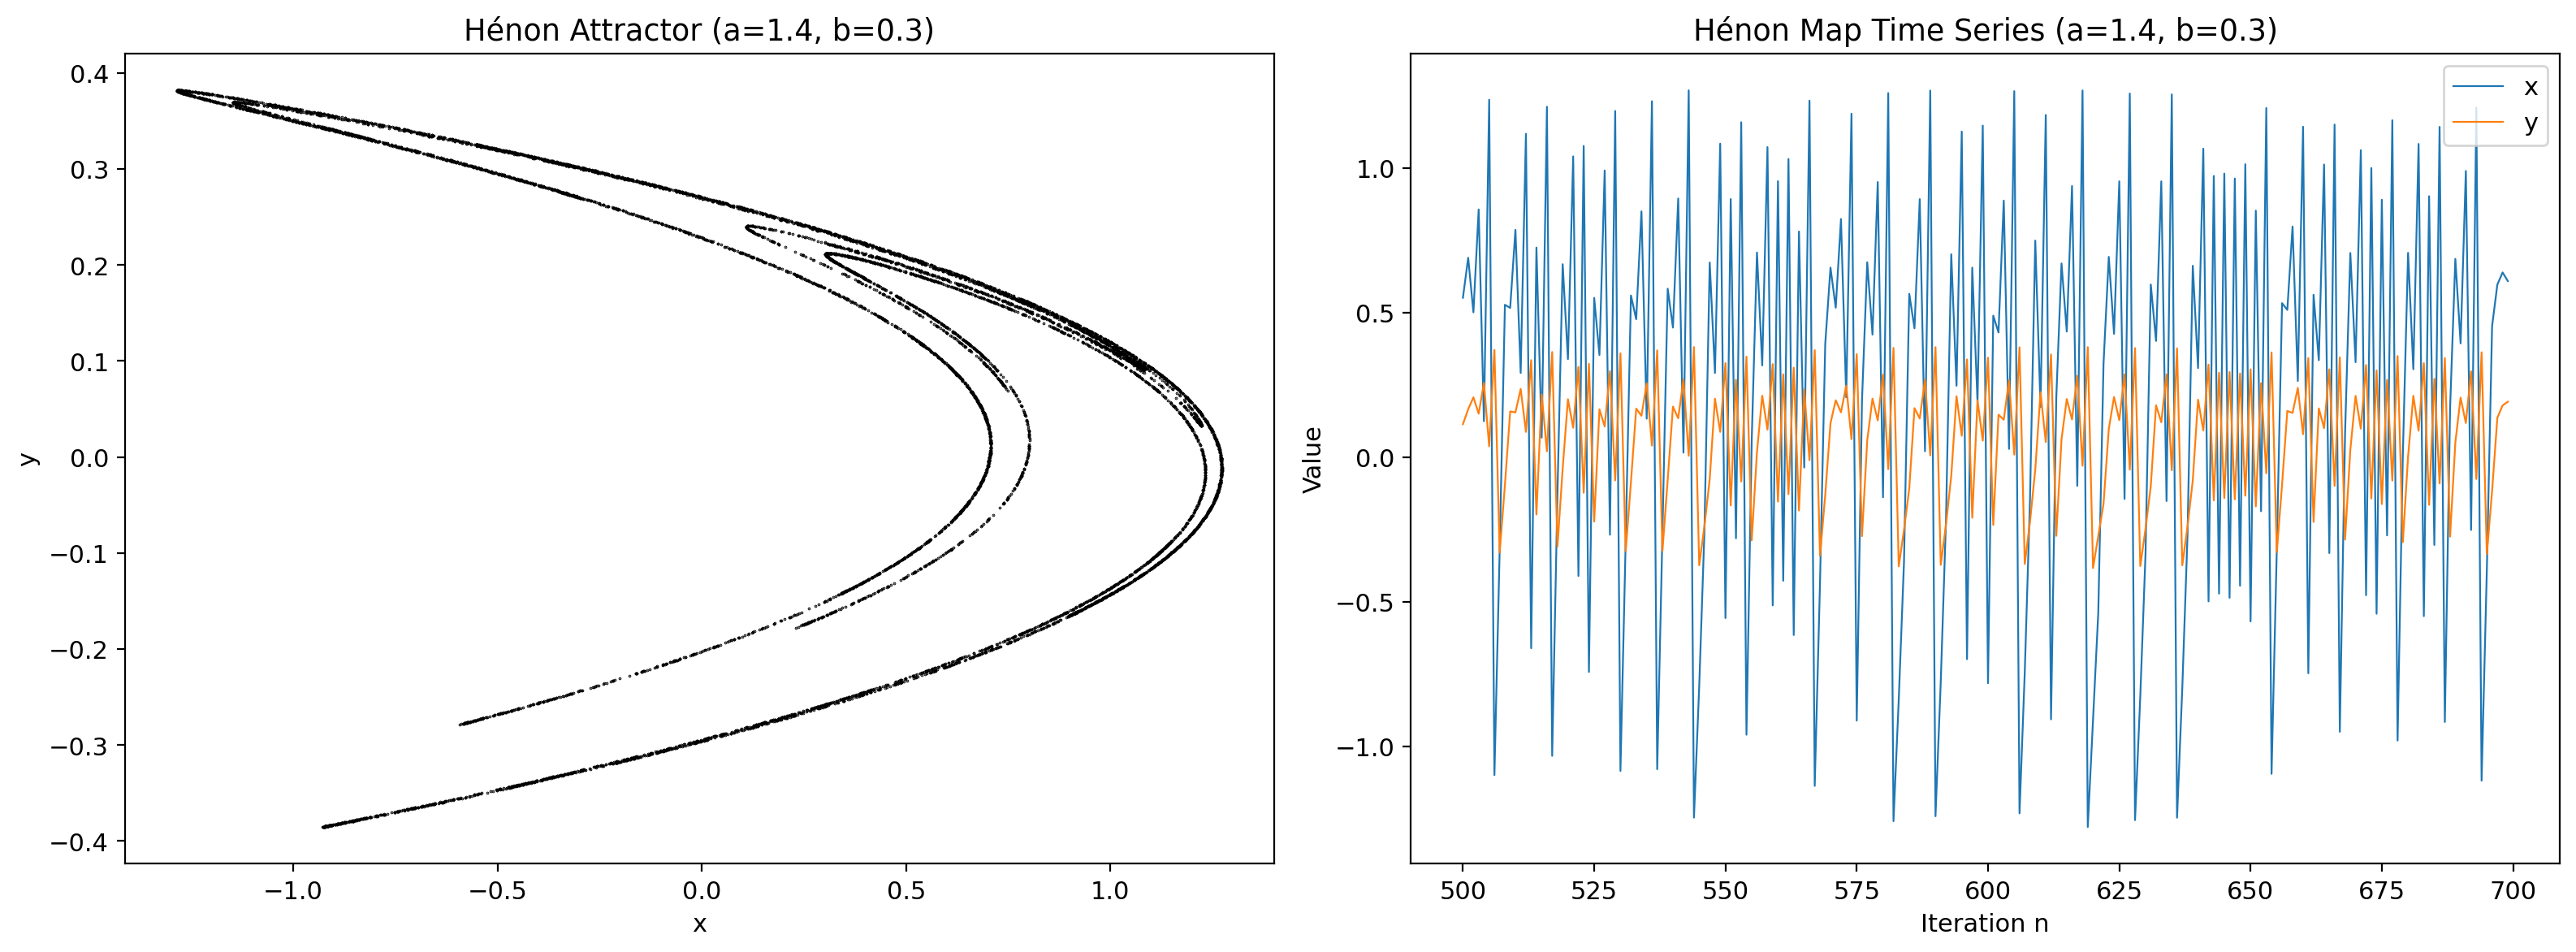
\includegraphics[width=0.95\textwidth]{henon_attractor_timeseries.png}
    \caption{H\'enon attractor (left) and time series (right) at $a=1.4$, $b=0.3$.}
    \label{fig:henon}
\end{figure}

The bifurcation diagram (Fig.~\ref{fig:henon_bif}) sweeps $a \in [1.0, 1.4]$ with $b = 0.3$ fixed. Period-doubling routes to chaos are visible, similar in structure to the logistic map but with additional complexity from the two-dimensional dynamics. Some parameter values cause orbits to diverge to infinity.

\begin{figure}[H]
    \centering
    
\includegraphics[width=0.85\textwidth]{henon_bifurcation.png}
    \caption{H\'enon map bifurcation diagram ($b = 0.3$).}
    \label{fig:henon_bif}
\end{figure}

%% ===== PART B =====
\section{Part B --- Continuous Chaotic Systems}

All continuous systems were integrated using \texttt{scipy.integrate.solve\_ivp} with the RK45 adaptive method (\texttt{rtol}=$10^{-10}$, \texttt{atol}=$10^{-12}$).

\subsection{Lorenz System}

\begin{table}[H]
\centering
\caption{Lorenz system settings.}
\begin{tabular}{ll}
\toprule
\textbf{Setting} & \textbf{Value} \\
\midrule
Equations & $\dot{x} = \sigma(y-x)$, $\dot{y} = x(\rho-z)-y$, $\dot{z} = xy - \beta z$ \\
Parameters & $\sigma = 10$, $\rho = 28$, $\beta = 8/3$ \\
Initial condition & $(1, 1, 1)$ \\
$dt$ / $T$ & $0.01$ / $50$ \\
\bottomrule
\end{tabular}
\end{table}

The 3D phase-space trajectory (Fig.~\ref{fig:lorenz_phase}) forms the well-known two-winged butterfly attractor. The trajectory spirals around one lobe before switching unpredictably to the other. Time series (Fig.~\ref{fig:lorenz_ts}) confirm the irregular switching in $x(t)$ and $y(t)$, while $z(t)$ remains strictly positive.

\begin{figure}[H]
    \centering
    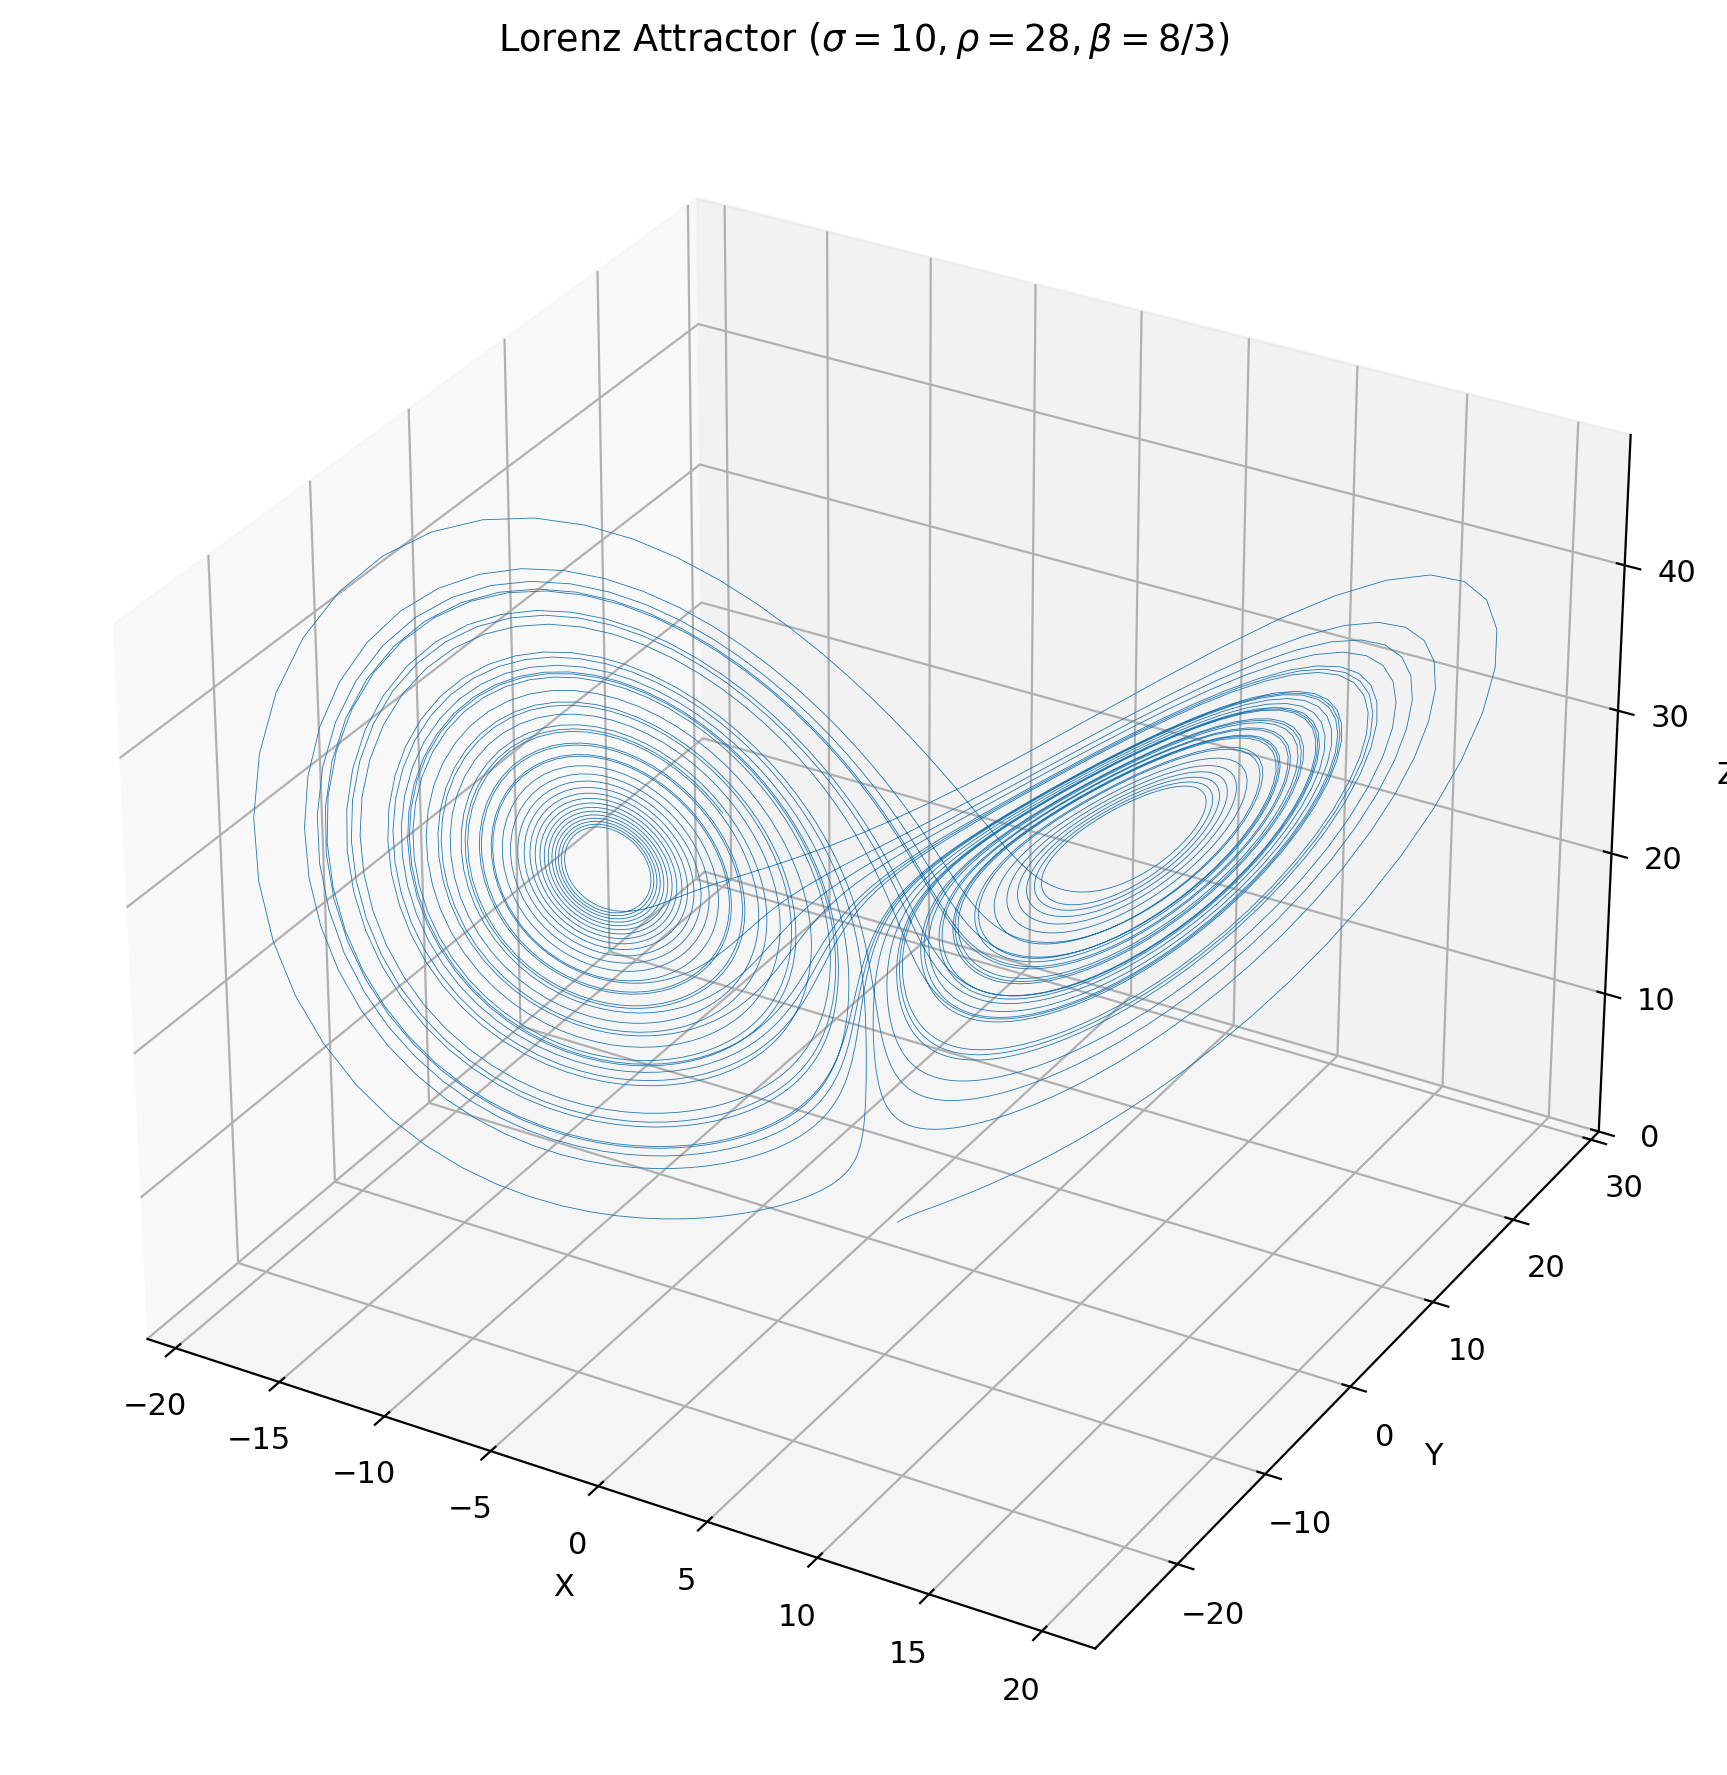
\includegraphics[width=0.75\textwidth]{lorenz_phase.png}
    \caption{Lorenz attractor in 3D phase space.}
    \label{fig:lorenz_phase}
\end{figure}

\begin{figure}[H]
    \centering
    
\includegraphics[width=0.85\textwidth]{lorenz_timeseries.png}
    \caption{Lorenz system time series.}
    \label{fig:lorenz_ts}
\end{figure}

\subsection{R\"ossler System}

\begin{table}[H]
\centering
\caption{R\"ossler system settings.}
\begin{tabular}{ll}
\toprule
\textbf{Setting} & \textbf{Value} \\
\midrule
Equations & $\dot{x} = -y-z$, $\dot{y} = x+ay$, $\dot{z} = b+z(x-c)$ \\
Parameters & $a = 0.2$, $b = 0.2$, $c = 5.7$ \\
Initial condition & $(1, 1, 1)$ \\
$dt$ / $T$ & $0.01$ / $300$ \\
\bottomrule
\end{tabular}
\end{table}

The R\"ossler attractor (Fig.~\ref{fig:rossler_phase}) exhibits a single-scroll spiral in the $x$-$y$ plane, with occasional upward excursions in $z$ (the reinjection mechanism). Unlike the Lorenz system's double-scroll structure, R\"ossler produces a simpler topology with one positive Lyapunov exponent.

\begin{figure}[H]
    \centering
    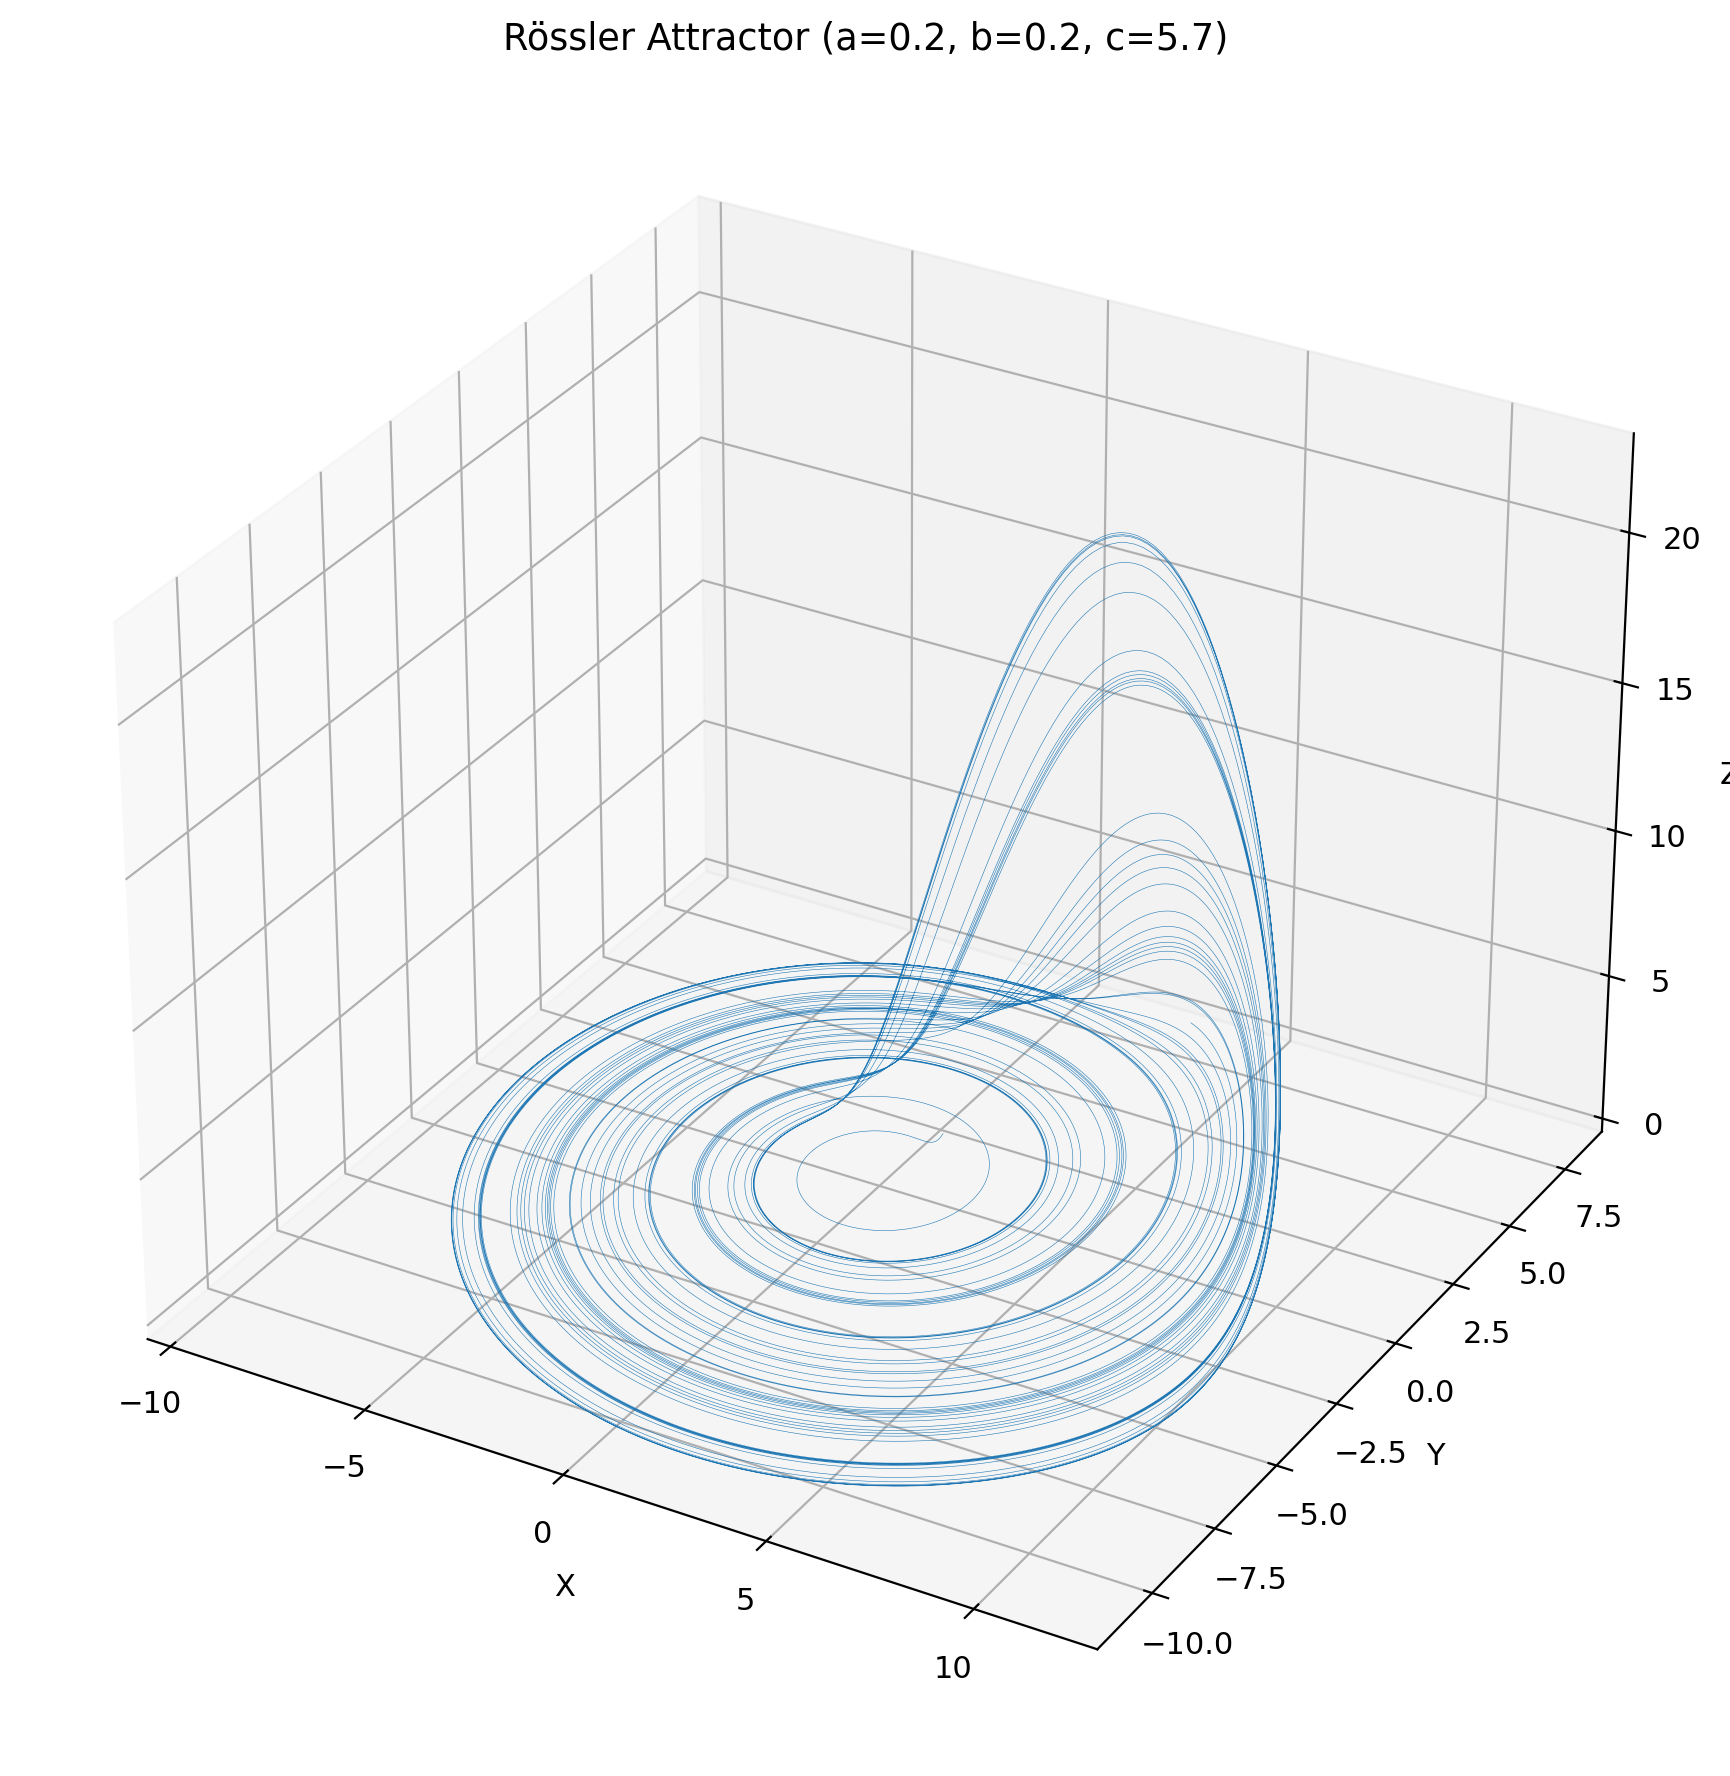
\includegraphics[width=0.75\textwidth]{rossler_phase.png}
    \caption{R\"ossler attractor.}
    \label{fig:rossler_phase}
\end{figure}

\begin{figure}[H]
    \centering
    
\includegraphics[width=0.85\textwidth]{rossler_timeseries.png}
    \caption{R\"ossler system time series.}
    \label{fig:rossler_ts}
\end{figure}

\subsection{Chen System}

\begin{table}[H]
\centering
\caption{Chen system settings.}
\begin{tabular}{ll}
\toprule
\textbf{Setting} & \textbf{Value} \\
\midrule
Equations & $\dot{x} = a(y-x)$, $\dot{y} = (c-a)x - xz + cy$, $\dot{z} = xy - bz$ \\
Parameters & $a = 35$, $b = 3$, $c = 28$ \\
Initial condition & $(-0.1, 0.5, -0.6)$ \\
$dt$ / $T$ & $0.002$ / $50$ \\
\bottomrule
\end{tabular}
\end{table}

The Chen attractor (Fig.~\ref{fig:chen_phase}) produces a double-scroll structure reminiscent of the Lorenz attractor but wider and more symmetric. Despite sharing the same $\dot{x} = a(y-x)$ form, the different coupling in $\dot{y}$ and $\dot{z}$ produces a distinct attractor geometry.

\begin{figure}[H]
    \centering
    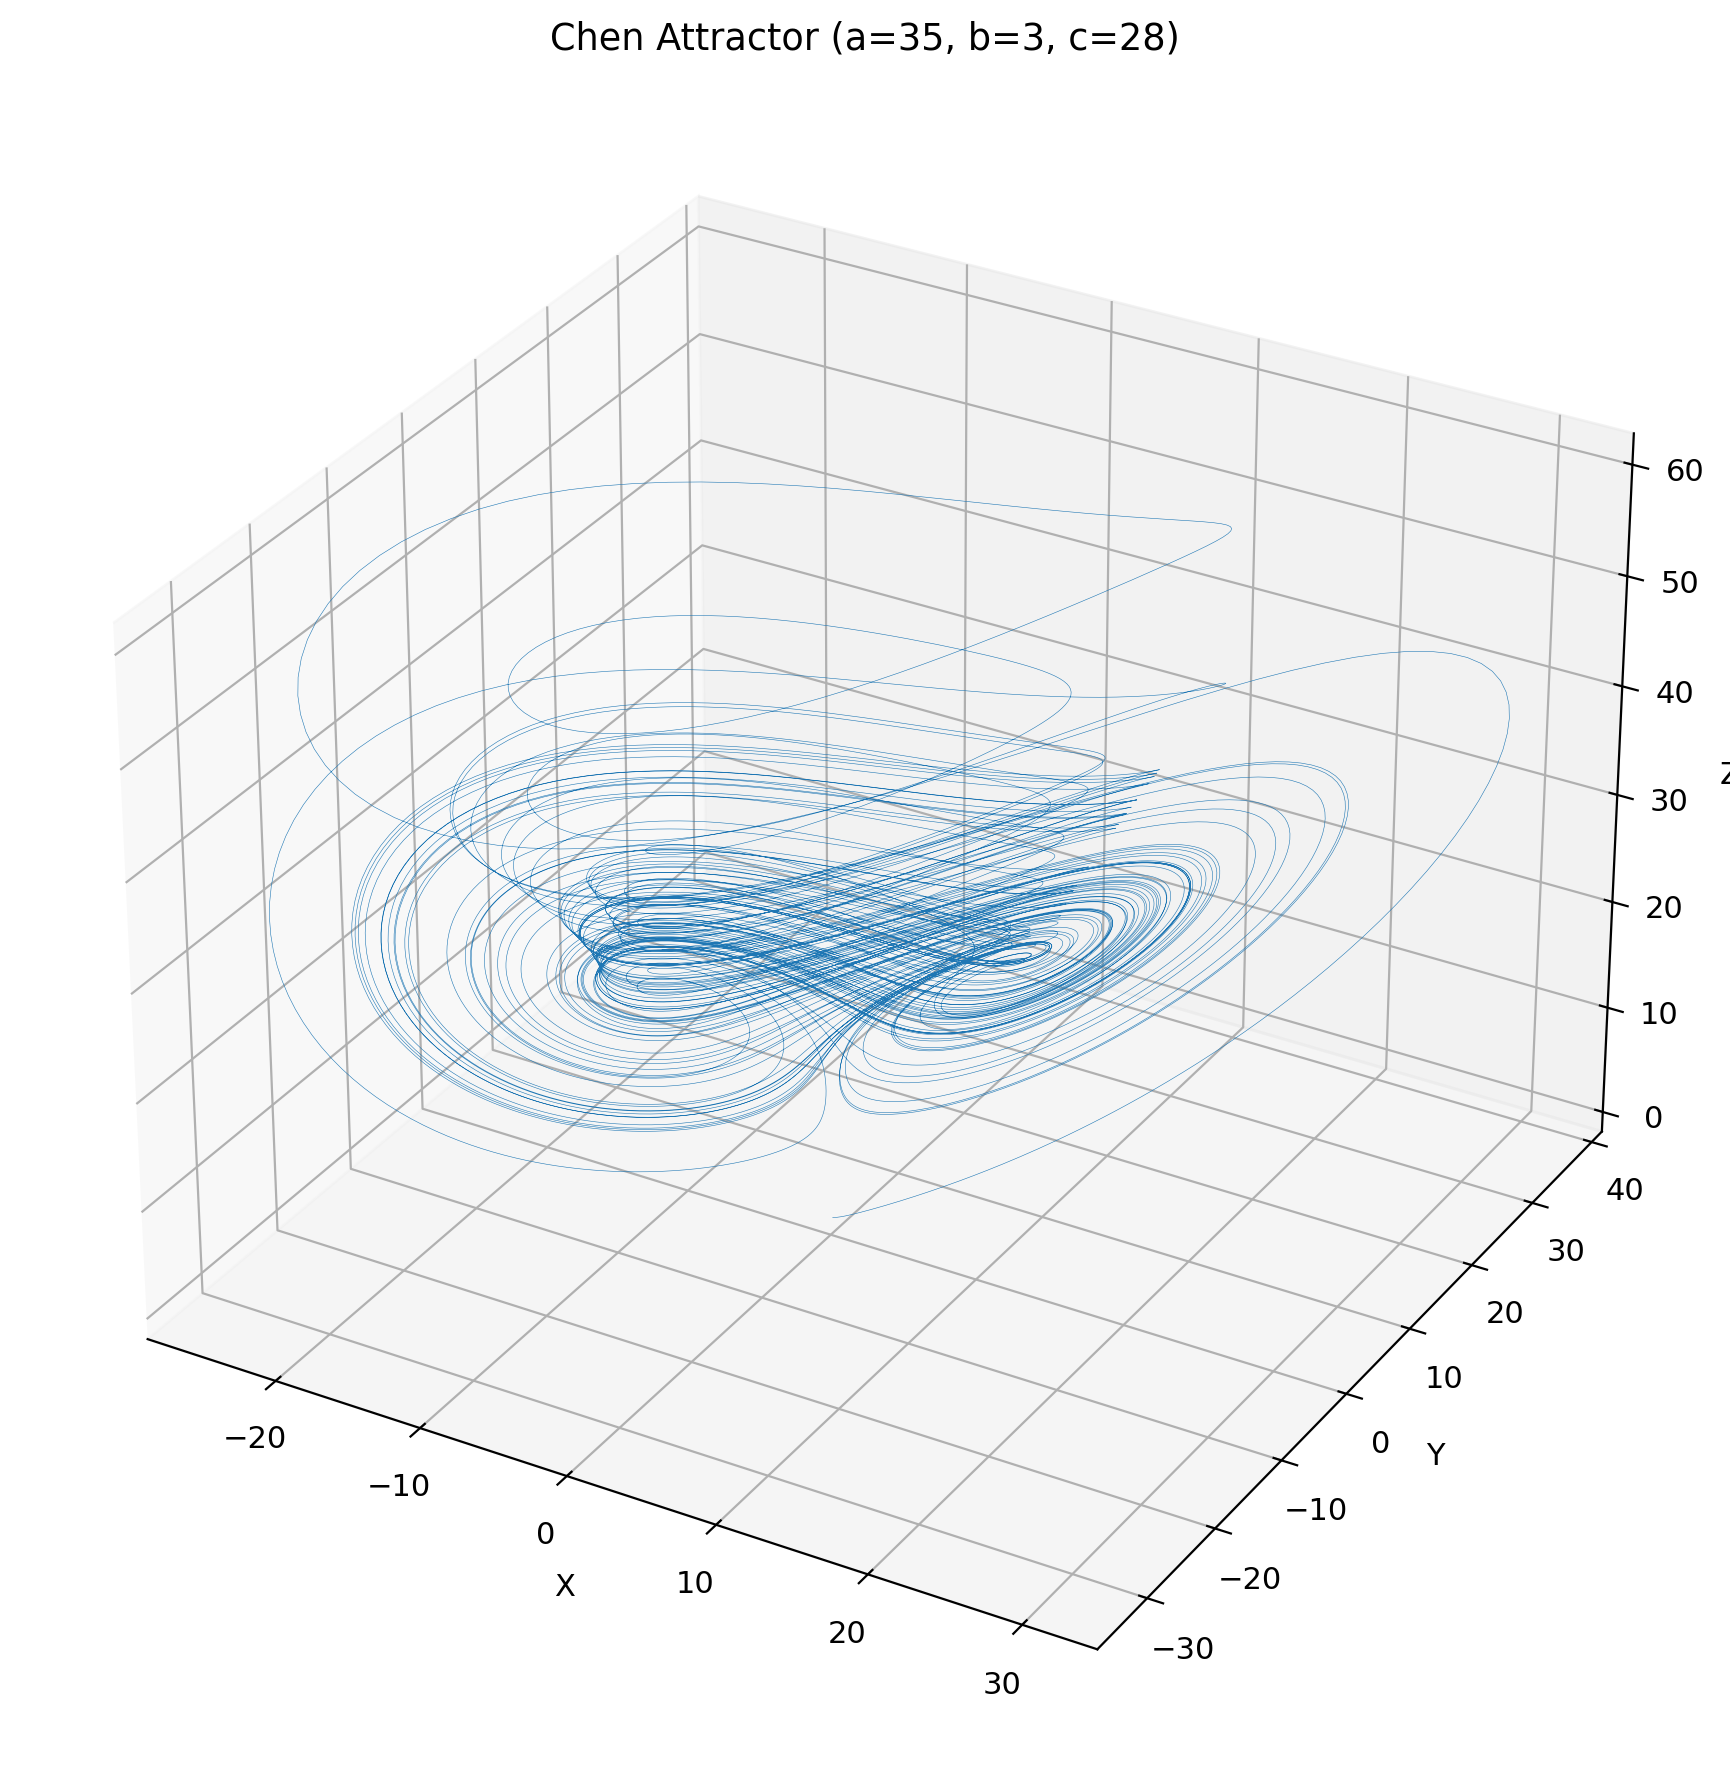
\includegraphics[width=0.75\textwidth]{chen_phase.png}
    \caption{Chen attractor.}
    \label{fig:chen_phase}
\end{figure}

\begin{figure}[H]
    \centering
    
\includegraphics[width=0.85\textwidth]{chen_timeseries.png}
    \caption{Chen system time series.}
    \label{fig:chen_ts}
\end{figure}

\subsection{Hyperchaotic R\"ossler System}

\begin{table}[H]
\centering
\caption{Hyperchaotic R\"ossler system settings.}
\begin{tabular}{ll}
\toprule
\textbf{Setting} & \textbf{Value} \\
\midrule
Equations & $\dot{x} = -y-z$, $\dot{y} = x+ay+w$, $\dot{z} = b+xz$, $\dot{w} = -cz+dw$ \\
Parameters & $a = 0.25$, $b = 3$, $c = 0.5$, $d = 0.05$ \\
Initial condition & $(-10, -6, 0, 10)$ \\
$dt$ / $T$ & $0.01$ / $250$ \\
\bottomrule
\end{tabular}
\end{table}

The 4D hyperchaotic R\"ossler system requires phase-space projections for visualization. Figure~\ref{fig:hyper_proj} shows the $x$-$y$, $x$-$z$, and $y$-$w$ projections. Compared to the standard R\"ossler attractor, the trajectories fill space more densely --- a signature of hyperchaos, where two or more positive Lyapunov exponents cause divergence in multiple independent directions simultaneously.

\begin{figure}[H]
    \centering
    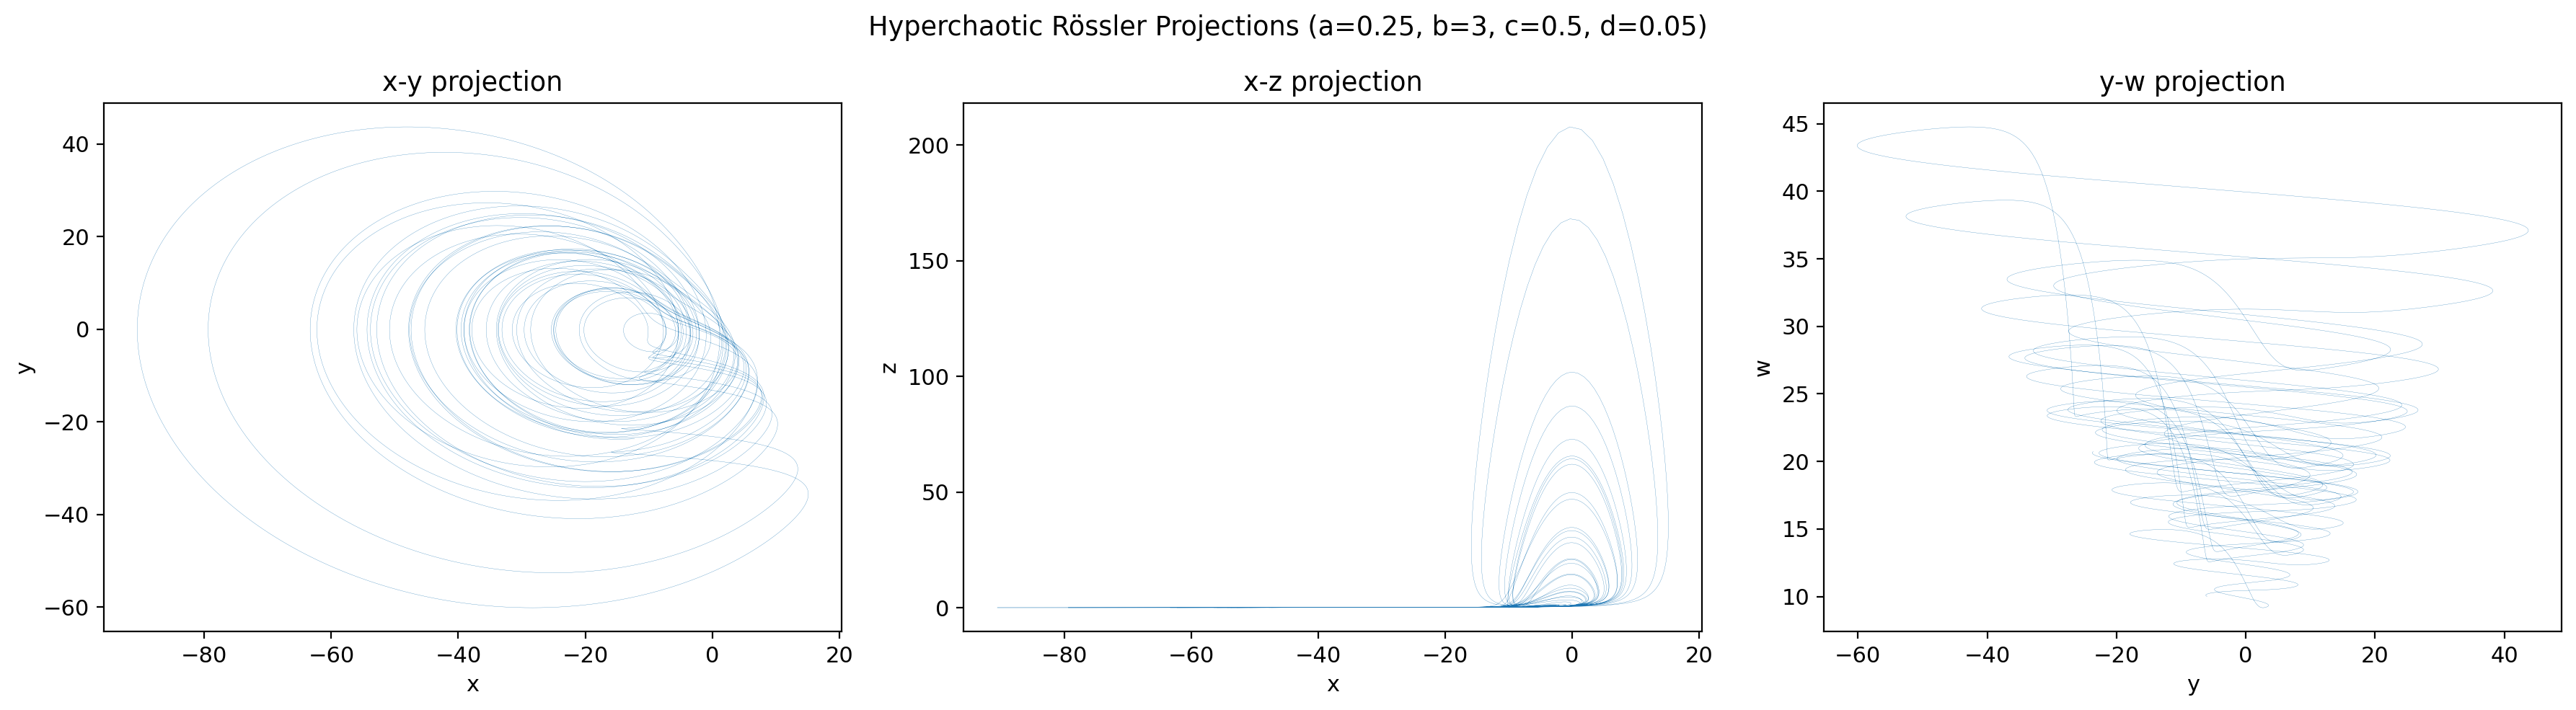
\includegraphics[width=\textwidth]{hyper_rossler_projections.png}
    \caption{Hyperchaotic R\"ossler phase-space projections.}
    \label{fig:hyper_proj}
\end{figure}

\begin{figure}[H]
    \centering
    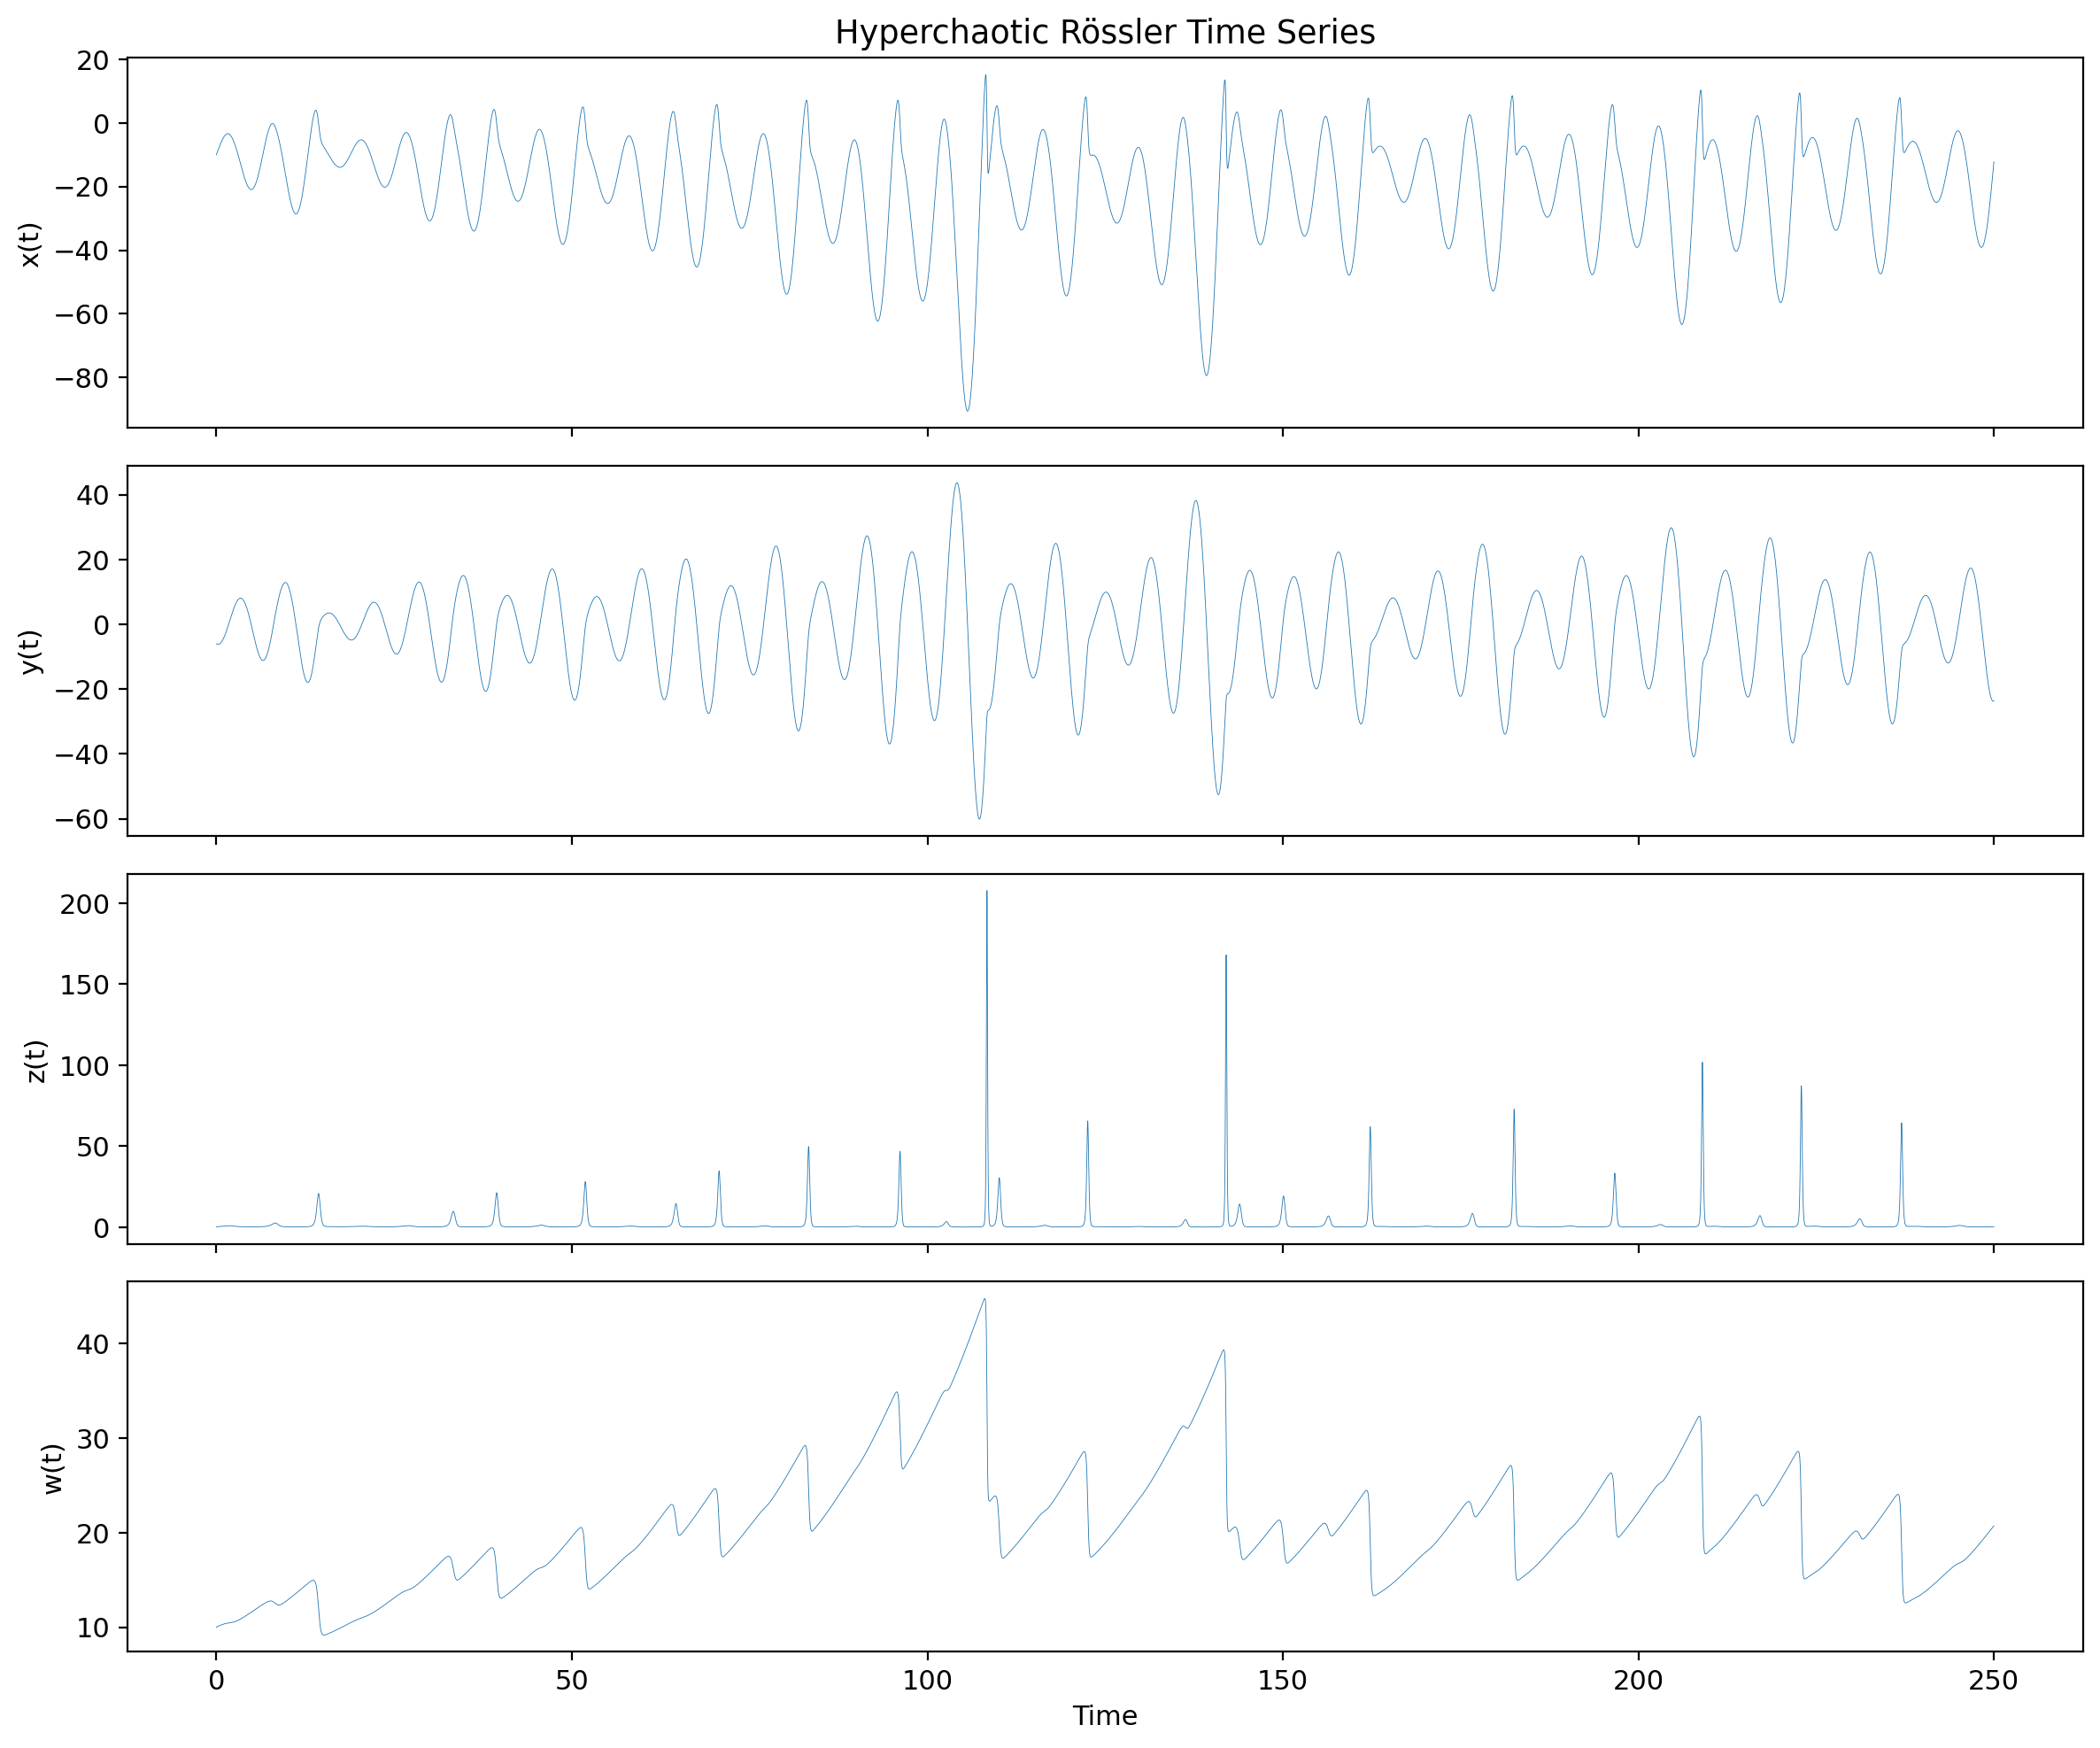
\includegraphics[width=0.85\textwidth]{hyper_rossler_timeseries.png}
    \caption{Hyperchaotic R\"ossler time series (all four state variables).}
    \label{fig:hyper_ts}
\end{figure}

%% ===== PART C =====
\section{Part C --- Sensitivity Analysis}

\subsection{Parameter Sweep: Lorenz $\rho$-Sweep}

Figure~\ref{fig:rho_sweep} shows the local maxima of $z(t)$ as $\rho$ is swept from 0 to 30 (with $\sigma = 10$, $\beta = 8/3$ fixed). For small $\rho$, the system converges to a stable fixed point (origin). Around $\rho \approx 1$, a pitchfork bifurcation creates two symmetric fixed points. Near $\rho \approx 24.7$, a Hopf bifurcation destabilizes these fixed points, and the system transitions through periodic windows into fully developed chaos at $\rho = 28$.

\begin{figure}[H]
    \centering
    
\includegraphics[width=0.85\textwidth]{lorenz_rho_sweep.png}
    \caption{Lorenz $\rho$-sweep: local maxima of $z(t)$ vs.\ $\rho$.}
    \label{fig:rho_sweep}
\end{figure}

\subsection{Step-Size Sensitivity}

The Lorenz system was re-simulated at the standard chaotic parameters using a \textbf{fixed-step RK4} integrator with $dt = 0.001$ (fine), $dt = 0.01$ (baseline), and $dt = 0.05$ (coarse). All three simulations start from the identical initial condition $(1, 1, 1)$.

As shown in Fig.~\ref{fig:stepsize_xt}, all three trajectories agree closely for the first $\sim$15--20 time units, after which they progressively diverge. The coarser step size ($dt = 0.05$) diverges earliest. The log-scale divergence plot (Fig.~\ref{fig:stepsize_div}) reveals approximately exponential growth of the trajectory difference, consistent with the positive Lyapunov exponent of the system.

This demonstrates that in chaotic systems, numerical truncation errors at each integration step act as effective perturbations to the initial condition. Because nearby trajectories separate exponentially, even small differences in numerical accuracy lead to completely uncorrelated trajectories after a finite time. The $dt = 0.01$ step size is sufficient to resolve the attractor's geometry accurately, while $dt = 0.05$ begins to distort the attractor structure.

\begin{figure}[H]
    \centering
    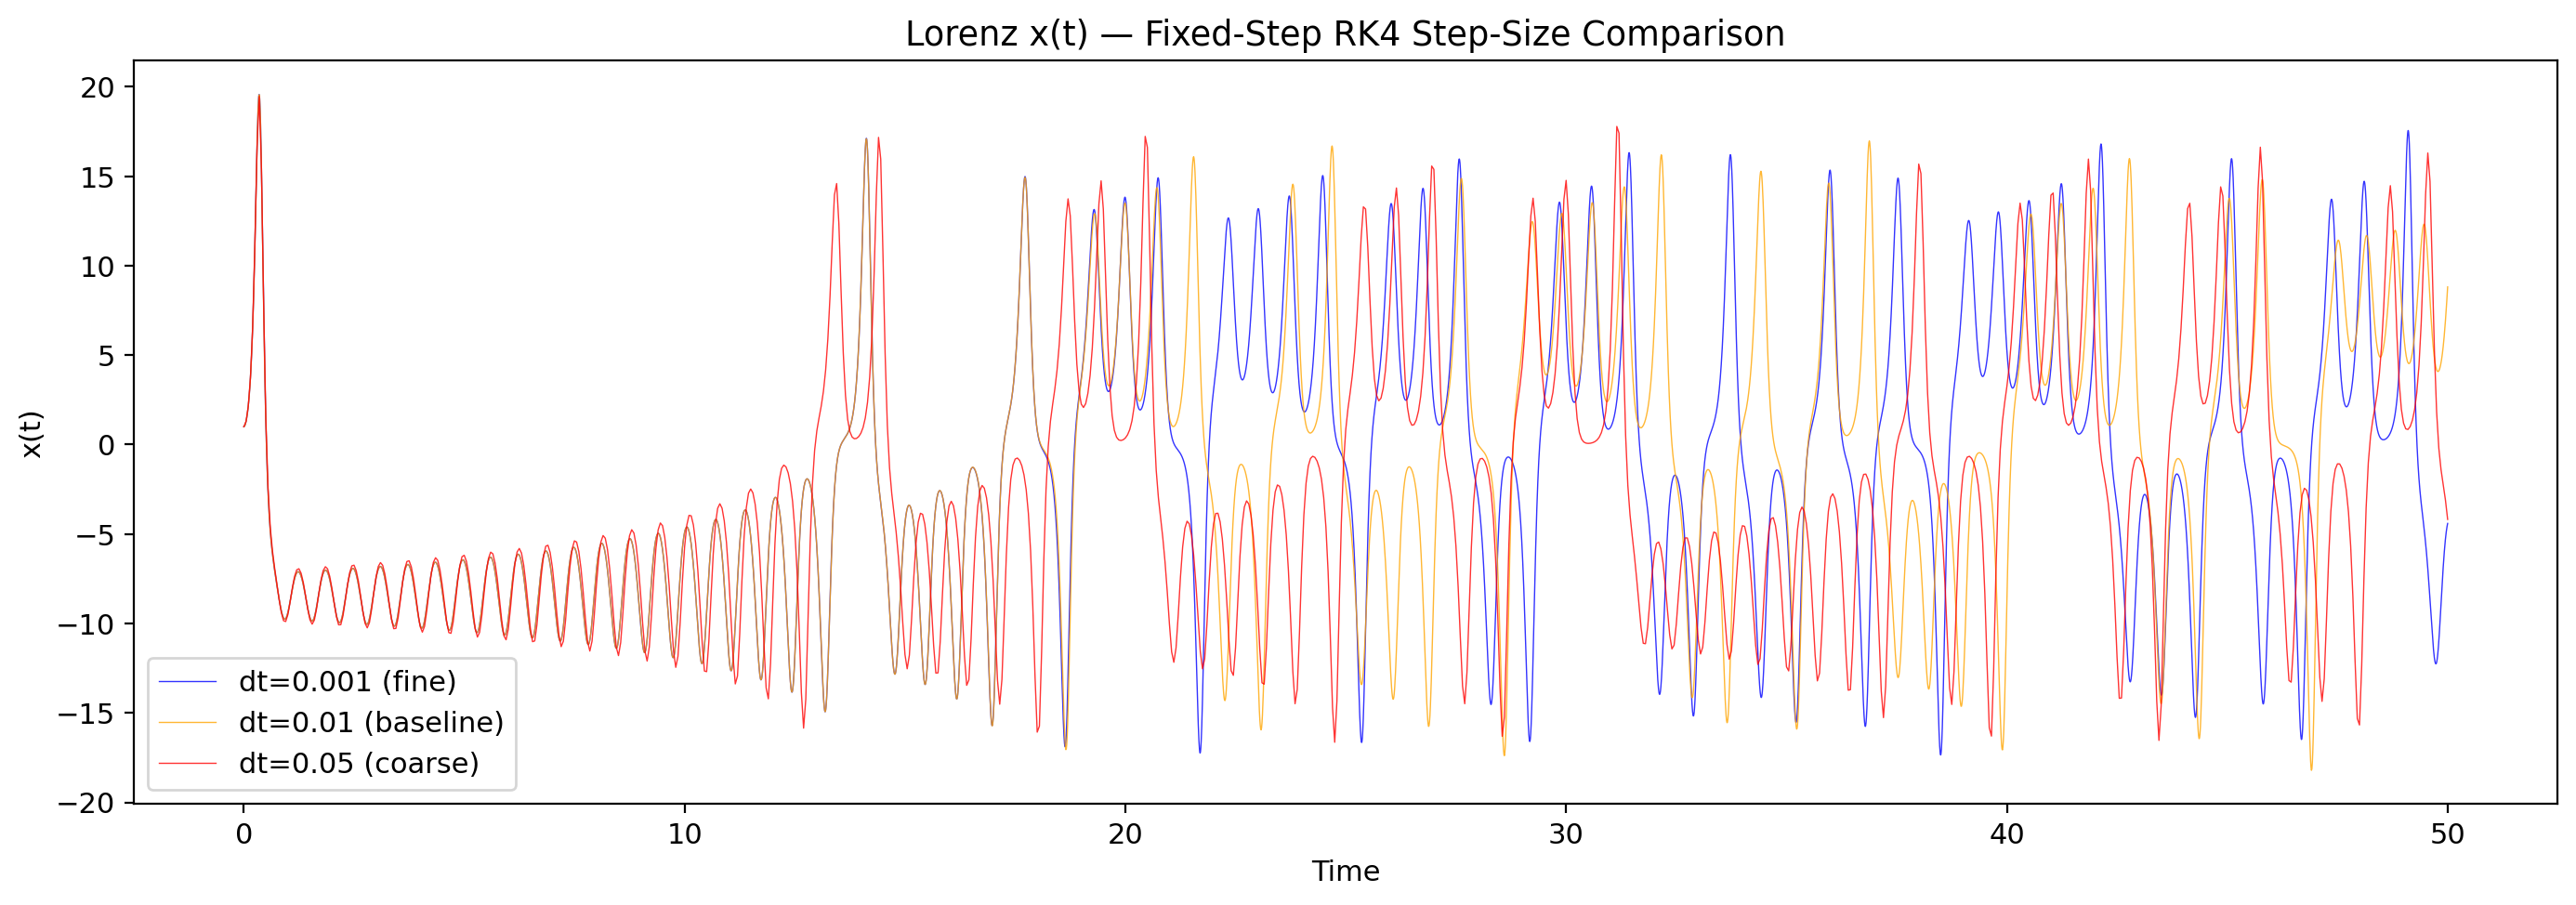
\includegraphics[width=0.9\textwidth]{stepsize_xt_overlay.png}
    \caption{Lorenz $x(t)$ for three RK4 step sizes.}
    \label{fig:stepsize_xt}
\end{figure}

\begin{figure}[H]
    \centering
    
\includegraphics[width=0.9\textwidth]{stepsize_phase_overlay.png}
    \caption{Lorenz 3D phase space overlay for three step sizes.}
    \label{fig:stepsize_phase}
\end{figure}

\begin{figure}[H]
    \centering
    
\includegraphics[width=0.9\textwidth]{stepsize_divergence.png}
    \caption{Trajectory divergence $|x_{dt}(t) - x_{\mathrm{fine}}(t)|$ on a log scale.}
    \label{fig:stepsize_div}
\end{figure}

%% ===== CONCLUSION =====
\section{Conclusion}

Discrete chaotic systems (logistic and H\'enon maps) demonstrate that chaos can emerge from simple iterative rules in as few as one dimension. Continuous chaotic systems (Lorenz, R\"ossler, Chen) require a minimum of three dimensions and exhibit richer dynamics including strange attractors with complex geometric structure. Both classes share the defining property of sensitive dependence on initial conditions, as confirmed by the step-size sensitivity analysis.

The transition from chaotic to hyperchaotic behavior, illustrated by the 4D R\"ossler system, involves the appearance of a second positive Lyapunov exponent. This causes trajectories to diverge in multiple independent directions simultaneously, producing denser, more space-filling attractors that are fundamentally harder to predict or reconstruct from partial observations.

\end{document}
